% !TeX root = orbits.tex
% !TeX Program=pdfLaTeX

\part{Ellipses}

%%%%%%%%%%%%%%%%%%%%%%%%%%%%%%%%%%%%%%%%%%%%%%%%%%%%%%%%%%%%%


\chapter{Definitions of ellipses}\label{s.definitions}

\section{Four definitions of an ellipse}

Ellipses can be defined analytically as the locus of points in the Cartesian plane satisfying a certain equation. Geometrically, an ellipse is defined by selecting two points, the foci, and defining the curve as the locus of points such that the sum of the distances to the foci is constant. Less well-known is the definition in terms of a focus and a directrix, but this was fundamental to the study of conic sections. Finally, we give the parametric representation of an ellipse that will be used in one of the proofs.

\subsection*{Analytic geometry}

\begin{definition}\label{def.analytic}
Let $a,b$ be positive real numbers. An \emph{ellipse} is the locus of the points $P=(x,y)$ in the Cartesian plane that satisfy the equation\footnote{This equation holds for ellipses centered at the origin, whose axes are on the axes of the Cartesian plane.}
\begin{equation}
\frac{x^2}{a^2}+\frac{y^2}{b^2}=1\,.\label{eqn.ellipse-formula}
\end{equation}
\end{definition}

%%%%%%%%%%%%%%%%%%%%%%%%%%%%%%%%%%%%%%%%%%%%%%%%%%%%%%%%%%%%%

\subsection*{Two foci}
\begin{definition}\label{def.two-foci}
Let $S$ and $H$ be two points in the Cartesian plane such that $SH=2c\geq 0$ and choose $a$ such that $2a> 2c$ (Figure~\ref{f.two-foci}). An \emph{ellipse} is the locus of all points $P$ such that $SP+PH=2a$. If $c=0$ the locus is a \emph{circle}.
\end{definition}

%%%%%%%%%%%%%%%%%%%%%%%%%%%%%%%%%%%%%%%%%%%%%%%%%%%%%%%%%%%%%

\begin{figure}[b]
\begin{minipage}{.48\textwidth}
\begin{center}
\begin{tikzpicture}
\clip (-3.5,-2.5) rectangle +(7,5);
% Size and center of the ellipse
\def\a{3}
\def\b{2}
\def\angle{70}
\pic{ellipse={{\a}/{\b}}};
% Label distances from center to foci by c
\path (F1) -- node[below] {$c$} (O) -- node[below] {$c$} (F2);
% Select an arbitrary point on the ellipse and draw lines to the foci
\pic{point-on-ellipse={{\a}/{\b}/{\angle}}};
\draw (F1) -- node[fill=white] {$a'$} (P) -- node[fill=white] {$a-a'$} (F2);
\node[above] at (Top) {$B$};
\node[below] at (Bot) {$B'$};
\node[right] at (Right) {$A$};
\node[left] at (Left) {$A'$};
\node[below left,xshift=3pt,yshift=-2pt] at (O) {$O$};
\node[below] at (F1) {$S$};
\node[below] at (F2) {$H$};
\end{tikzpicture}
\caption{The foci $S,H$ and the lengths $a$, $c$}\label{f.two-foci}
\end{center}
\end{minipage}
\hspace*{2pt}
\begin{minipage}{.48\textwidth}
\begin{center}
\begin{tikzpicture}
\clip (-3.5,-2.5) rectangle +(7,5);
% Ellipse
\def\a{3}
\def\b{2}
\pic{ellipse={{\a}/{\b}}};

% Label nodes
\node[above] at (Top) {$B$};
\node[below] at (Bot) {$B'$};
\node[right] at (Right) {$A$};
\node[left] at (Left) {$A'$};
\node[below] at (F1) {$S$};
\node[below] at (F2) {$H$};
\node[below left,xshift=3pt,yshift=-2pt] at (O) {$O$};

% Label segments
\path (Bot) --  
  node[left,yshift=-8pt] {$b$} (O) -- node[left] {$b$} (Top);
\path (F1) -- node[below] {$c$} (O) -- node[below] {$c$} (F2);
\draw (F1) -- node[above] {$a$} (Top) -- node[above] {$a$} (F2);

% Indicates distances along the major axis
\draw[<->] ($(O)+(0,-20pt)$) -- node[fill=white] {$a$} ($(Right)+(0,-20pt)$);
\draw[<->] ($(O)+(0,-20pt)$) -- node[fill=white] {$a$} ($(Left)+(0,-20pt)$);

\draw (O) rectangle +(6pt,6pt);
\end{tikzpicture}
\caption{The axes of an ellipse}
\label{f.ellipse-features}
\end{center}
\end{minipage}
\end{figure}

%%%%%%%%%%%%%%%%%%%%%%%%%%%%%%%%%%%%%%%%%%%%%%%%%%%%%%%%%%%%%

\begin{definition}\label{def.features}
Consider a line containing the segment $SH$ and $A,A'$ be the intersections of the line with the ellipse. $AA'$ is the \emph{major axis} of the ellipse. Let $O$ be the midpoint of $SH$. $AO,OA'$ are the \emph{semi-major axes} of the ellipse.

Consider a line perpendicular to $SH$ at $O$ and let $B,B'$ be its intersections with the ellipse. $BB'$ is the \emph{minor axis} of the ellipse and $BO,OB'$ are the \emph{semi-minor axes} of the ellipse.
\end{definition}

\begin{theorem}(Figure~\ref{f.ellipse-features})\label{thm.ellipses-features}
\begin{enumerate}
\item $SB=HB=a$.
\item $AO=OA'=a$.
\item $BO=OB'$. (Label $BO=OB'$ by $b$.)
\end{enumerate}
\end{theorem}

\begin{proof}
\begin{enumerate}
\item $\triangle SBO\cong\triangle HBO$ by side-angle-side  so $SB=HB$. Since $B$ is on the ellipse, $SB+HB=2a$ and $SB=HB=a$ follows. 
\item Since $A$ is on the ellipse, $2a = AS+HA = (AO-c)+(AO+c)=2AO$,
so $AO=a$. $OA'=a=AO$ follows by symmetry.
\item $BO=OB'$ follows from $\triangle SBO\cong\triangle SB'O$.\hqed
\end{enumerate}
\end{proof}
%%%%%%%%%%%%%%%%%%%%%%%%%%%%%%%%%%%%%%%%%%%%%%%%%%%%%%%%%%%%%

\begin{figure}[t]
\begin{center}
\begin{tikzpicture}
\clip (-.5,-2) rectangle +(7,4);

% Construct the directrix and the focus
\coordinate (X) at (0,0);
\node[left] at (X) {$X$};
\draw[name path=directrix] ($(X)+(0,2)$) --
  node[left,near start] {$d$} ($(X)+(0,-2)$);
\coordinate (S) at (3,0);
\node[below] at (S) {$S$};

% Locate the vertices with eccentricity 1/2
\coordinate (A) at (2,0);
\node[below] at (A) {$A$};
\coordinate (AP) at (6,0);
\node[below] at (AP) {$A'$};

% draw the major axis
\draw  (AP) -- node[above] {$3$} (S) -- 
  node[above left] {$1$} (A) -- node[above] {$2$} (X);

%\vertexsm{X};
\vertexsm{S};
\vertexsm{A};
\vertexsm{AP};
\end{tikzpicture}
\end{center}
\caption{The elements of the definition of an ellipse}\label{f.ellipse-conic}
\end{figure}

%%%%%%%%%%%%%%%%%%%%%%%%%%%%%%%%%%%%%%%%%%%%%%%%%%%%%%%%%%%%%

\subsection*{Conic sections}

\begin{definition}\label{def.ellipse-conic}
Let $d$ be a line (the \emph{directrix}) and $S$ be a point (the \emph{focus}) not on the directrix. Let $0<e<1$ be a number (the \emph{eccentricity}). An \emph{ellipse} is the locus of points $P$ such that the ratio of  $PS$ to the distance of $P$ to the directrix is $e$.
\end{definition}
All the conic sections  are defined the same way and are distinguished by their eccentricity: $e<1$ for an ellipse, $e=1$ for a parabola and $e>1$ for a hyperbola.

\begin{definition}\label{def.vertex}
Let $X$ be the intersection of the perpendicular to the directrix from $S$. $A$ on $SX$ is a \emph{vertex} of the ellipse if $SA/AX=e$ (in Figure~\ref{f.ellipse-conic}, $e=1/2$).
\end{definition}

%%%%%%%%%%%%%%%%%%%%%%%%%%%%%%%%%%%%%%%%%%%%%%%%%%%%%%%%%%%%%

\subsection*{Generating the conic-section ellipse}

Definition~\ref{def.ellipse-conic} is non-constructive. It states that the ellipse is the locus of points satisfying a certain property, but aside from the vertices we have not constructed any such points. Here we show how to construct any of the points on the ellipse.

Select an \emph{arbitrary} point $E$ on the directrix and construct lines from $E$ through $A$ and $S$. The line through $S$ will make an angle $\alpha$ with $SX$. Construct a line from $S$ at the \emph{same angle} $\alpha$ from $ES$ and let its intersection with $EA$ be $P$. Construct the perpendicular from $P$ to the directrix and let $K$ be its intersection with the directrix. Let $L$ be the intersection of $KP$ with $ES$ (Figure~\ref{f.construct}). 

%%%%%%%%%%%%%%%%%%%%%%%%%%%%%%%%%%%%%%%%%%%%%%%%%%%%%%%%%%

\begin{figure}[b]
\begin{center}
\begin{tikzpicture}

\clip (-.8,-2.2) rectangle +(10,4.5);

% Construct the directrix, the focus and the major axis
\coordinate (X) at (0,0);
\node[left] at (X) {$X$};
\draw[name path global=directrix] ($(X)+(0,2)$) --
  node[left,near start] {$d$} ($(X)+(0,-2)$);
\coordinate (S) at (3,0);
\node[below] at (S) {$S$};

% Locate a vertex
\coordinate (A) at (2,0);
\node[above left] at (A) {$A$};
\coordinate (AP) at (7,0);
\node[right] at ($(AP)+(1,0)$) {$N$};

% Find a convenient E and draw _paths_ to A and S
\path[name path=findE] (S) -- +(210:4);
\path [name intersections = {of = findE and directrix, by = {E} }];
\node[left] at (E) {$E$};
\path[name path=EA] (E) -- ($(E)!2.3!(A)$);
\path[name path=ES] (E) -- ($(E)!2.3!(S)$);

% Locate P by drawing a path with the same angle
\path[name path=SP] (S) -- +(60:3);
\path [name intersections = {of = EA and SP, by = {P} }];
\node[above] at (P) {$P$};
\draw (S) -- (P);

% Construct the perpendicular through P to the directrix
\path[name path=PK] (P) -- +(180:4.5);
\path [name intersections = {of = PK and directrix, by = {K} }];
\node[left] at (K) {$K$};
\draw[name path=PL] (K) -- ($(K)!1.8!(P)$);

% Locate L and label the segments
\path [name intersections = {of = PL and ES, by = {L} }];
\node[above] at (L) {$L$};
\path (S) -- node[left] {$b$} (P) -- node[above] {$b$} (L);

% Label the angles
\node[right,xshift=12pt,yshift=5pt] at (S) {$\alpha$};
\node[above right,xshift=6pt,yshift=8pt] at (S) {$\alpha$};
\node[below left,xshift=-12pt,yshift=1pt] at (L) {$\alpha$};

% Draw the colored triangles
\draw[red,very thick] (P) -- (L) -- (E) -- cycle;
\draw[blue,very thick] (E) -- (K) -- ($(P)+(-3pt,0)$) -- ($(E)+(0,3pt)$);

\draw (X) -- ($(AP)+(1,0)$);
\end{tikzpicture}
\end{center}
\caption{Constructing points on the ellipse}\label{f.construct}
\end{figure}

%%%%%%%%%%%%%%%%%%%%%%%%%%%%%%%%%%%%%%%%%%%%%%%%%%%%%%%%%%%%%

\begin{theorem}\label{thm.point-on-an-ellipse}
The point $P$ is on the ellipse.
\end{theorem}
\begin{proof}
$\angle PLS = \angle LSN=\alpha$ by alternate interior angles, so $\triangle LPS$ is isosceles and $PL=SP$. Since $PK\parallel SX$, $\triangle XEA\sim \triangle KEP$ and $\triangle AES\sim \triangle PEL$ are adjacent pairs of similar triangles, so
\[
\frac{PS}{PK}=\frac{PL}{PK}=\frac{SA}{AX}=e\,.
\]
Therefore, $P$ is on the ellipse.\hqed
\end{proof}

By choosing different points $E$ on the directrix, any point on the ellipse can be constructed.


\begin{definition}[Parametric representation]
Consider two concentric circles, one of radius $a$ (dashed blue) and one of radius $b$ (dotted red) (Figure~\ref{f.parametric}). An \emph{ellipse} is the locus of points $P=(x,y)$ such that
\[
(x,y)= (a\cos t,\, y = b \sin t)\,,
\]
for $0\le t < 2\pi$.
\end{definition}
The parameter $t$ is \emph{not} the angle of $P$ relative to the positive $x$-axis. Construct the perpendicular through $P$ to the minor axis and let $P_I$ be its intersection with the inner circle so that $CP_I$ defines an angle $t$.  Extend $C_I$ until it intersects the outer circle at $P_O$. The parametric representation of $P$ is computed from the lengths of the axes and trigonometry functions of $t$.

%%%%%%%%%%%%%%%%%%%%%%%%%%%%%%%%%%%%%%%%%%%%%%%%%%%%%%%%%%%%%

\begin{figure}[t]
\begin{center}
\begin{tikzpicture}
\clip (-3.1,-3.3) rectangle +(6.2,6.6);
% Size and center of the ellipse
\def\a{3}
\def\b{2}
\coordinate (C) at (0,0);
\node[below left,xshift=2pt] at (C) {$O$};

% Draw an ellipse and the inner and outer circles
\draw[name path=ellipse] (C) ellipse[x radius=\a,y radius= \b];
\draw[very thick,dotted,red,name path=outer] (C) circle[radius=\a];
\draw[thick,dashed,blue,name path=inner] (C) circle[radius=\b];

% Locate P on the ellipse
\path[name path=toP] (C) -- +(30:4);
\path [name intersections = {of = ellipse and toP, by = {P} }];

% Label the angle of CP
\node[above right,xshift=8pt,yshift=-2pt] at (C) {$t$};

% Draw major and minor axes
\draw[name path=yplus] (C) -- +(0,\a);
\draw (C) -- +(0,-\a);
\draw[name path=xplus] (C) -- +(\a,0);
\draw (C) -- +(-\a,0);

% Find intersection PI of line from center to P and the inner circle
\node[below right,xshift=-3pt,yshift=-4pt] at (P) {$P$};
\vertexsm{P};
\path[name path=horiz] (P) -- +(-\a,0);
\path [name intersections = {of = inner and horiz, by = {PI} }];

% Extend ray C->PI to outer circle and label intersection PO
\path[name path=ray] (C) -- ($(C) !1.7! (PI)$);
\path [name intersections = {of = outer and ray, by = {PO} }];

% Project PO on x axis
\path[thick,name path=horizPO] (PO) -- +(0,-\a);
\path [name intersections = {of = xplus and horizPO, by = {xint} }];
\draw (PO) -- (xint);
\draw[<->,style={shorten <= 2pt}] ($(C)+(0,-5pt)$) --
  node[below,xshift=-4pt] {$a\cos t$} ($(xint)+(0,-5pt)$);

% Project PI on y axis
\path [name intersections = {of = yplus and horiz, by = {yint} }];
\draw[<->] ($(C)+(-5pt,0)$) -- 
  node[left,xshift=1pt] {$b\sin t$} ($(yint)+(-5pt,0)$);
\draw (P) -- (yint);

% Draw blue and red lines from C to PI and PO
\draw[thick,blue] (C) -- (PI);
\draw[thick,red] (PI) -- (PO);

% Dots at vertices
\vertexsmcolor{PI}{blue};
\vertexsmcolor{PO}{red};
\node[below,yshift=-4pt] at (PI) {$P_I$};
\node[above right] at (PO) {$P_O$};
%\vertexsm{C};
%\vertexsm{P};

\end{tikzpicture}
\caption{Parametric representation of an ellipse}\label{f.parametric}
\end{center}
\end{figure}

%%%%%%%%%%%%%%%%%%%%%%%%%%%%%%%%%%%%%%%%%%%%%%%%%%%%%%%%%%%%%

\begin{figure}[b]
\begin{center}
\begin{tikzpicture}
\clip (-3.3,-2.1) rectangle +(6.6,4.2);

\def\a{3.2}
\def\b{2}
\pic{ellipse={{\a}/{\b}}};

\node[below] at (F1) {$S$};
\node[below right] at (F2) {$H$};
\draw (F1) -- (O) -- (F2);
\draw[name path=minor] (O) -- (Top);

\vertexsm{F1};
\vertexsmcolor{F2}{red};

% Draw latus rectum as intersections of perpendicular at H
%  with the ellipse
\path[name path=LR] ($(F2)+(0,-2.5)$) -- ($(F2)+(0,2.5)$);
\path [name intersections = {of = ellipse and LR, by = {LR1,LR2} }];
\draw[very thick,red] (LR1) -- (LR2);

% Label endpoint of the LR
\node[above] at (LR1) {$L_1$};
\node[below] at (LR2) {$L_2$};
\draw (F2) rectangle +(5pt,5pt);

% Length of LR
\draw[<->,dashed,thick] ($(LR1)+(-.3,0)$) --
  node[left,xshift=2pt,yshift=-8pt] {$L$} ($(LR2)+(-.3,0)$);
\end{tikzpicture}
\caption{The circumscribed circle and the latus rectum of an ellipse}\label{f.ellipse-latus-rectum-def}
\end{center}
\end{figure}


%%%%%%%%%%%%%%%%%%%%%%%%%%%%%%%%%%%%%%%%%%%%%%%%%%%%%%%%%%%%%

\section{The latus rectum and conjugate diameters}

The following two definitions are at the heart of Newton's proof.

\subsection*{The latus rectum}

\begin{definition}\label{def.ellipse-lr}
Consider a line through a focus of an ellipse that is perpendicular the major axis. Let its intersections with the ellipse be $L_1,L_2$. Then $L=L_1L_2$ is a \emph{latus rectum} of an ellipse (Figure~\ref{f.ellipse-latus-rectum-def}).\footnote{Usually, lines are denoted by lower-case letters, but $L$ for the latus rectum is the standard notation.}
\end{definition}

%%%%%%%%%%%%%%%%%%%%%%%%%%%%%%%%%%%%%%%%%%%%%%%%%%%%%%%%%%%%%

\subsection*{Conjugate diameters}

\begin{definition}\label{def.conjugate}
There are two equivalent definitions of conjugate diameters.
\begin{itemize}
\item Let $P$ be a point on an ellipse, $PG$ a diameter and let $t$ be the tangent to the ellipse at $P$. Diameter $DK$ is a \emph{conjugate diameter} if it is parallel to $t$ (Figure~\ref{f.ellipse-conj}).
\item Two diameters $PG$ and $DK$ are \emph{conjugate diameters} if the midpoints of chords ($D'K'$, $D''K''$) parallel to one diameter ($DK$) lie on another diameter ($PG$).
\end{itemize}
\end{definition}

%%%%%%%%%%%%%%%%%%%%%%%%%%%%%%%%%%%%%%%%%%%%%%%%%%%%%%%%%%%%%

\begin{figure}[t]
\begin{center}
\begin{tikzpicture}

\clip (-3.5,-2.5) rectangle +(8,5);

\def\a{3}
\def\b{2}
\def\angle{29}

\pic{ellipse={\a}/{\b}};
\pic{point-on-ellipse={\a}/{\b}/{\angle}};
\pic{tangent={\a}/{\b}/{\angle}};

\node[above] at (Top) {$B$};
\node[below] at (Bot) {$B'$};
\node[right,xshift=-2pt] at (Right) {$A$};
\node[left] at (Left) {$A'$};
\node[below left,xshift=3pt,yshift=-2pt] at (O) {$O$};

% Diameter from P through O
\draw[name path=pc] (P) -- ($(P)!2!(O)$) coordinate (G);
\node[left,yshift=-2pt] at (G) {$G$};

% Conjugate diameters from D through O
\draw[name path=cd] (O) -- +({90+\angle}:{\a} and {\b});
\path[name path=dk] (O) -- +({-90+\angle}:{\a} and {\b});
\path [name intersections = {of = cd and ellipse, by = {D} }];
\path [name intersections = {of = dk and ellipse, by = {K} }];
\node[above left] at (D) {$D$};
\node[below right] at (K) {$K$};
\draw (D) -- (K);

% Draw parallels to the tangent
\coordinate (PP) at ($(O)!.35!(G)$);
\path[name path=pp1] (PP) -- ++ ({-\a*3*sin(\angle)},{\b*3*cos(\angle)});
\path [name intersections = {of = pp1 and ellipse, by = {DP} }];
\path[name path=pp2] (PP) -- ++ ({\a*3*sin(\angle)},{-\b*3*cos(\angle)});
\path [name intersections = {of = pp2 and ellipse, by = {KP} }];
\draw[thick,dashed,name path=center1] (DP) node[above] {$D'$} -- 
  (KP) node[below right] {$K'$};

\coordinate (PPP) at ($(O)!.6!(P)$);
\path[name path=ppp1] (PPP) -- ++ ({-\a*3*sin(\angle)},{\b*3*cos(\angle)});
\path [name intersections = {of = ppp1 and ellipse, by = {DPP} }];
\path[name path=ppp2] (PPP) -- ++ ({\a*3*sin(\angle)},{-\b*3*cos(\angle)});
\path [name intersections = {of = ppp2 and ellipse, by = {KPP} }];
\draw[thick,dashed,name path=center2] (DPP) node[above] {$D''$} --
  (KPP) node[below right] {$K''$};

\path [name intersections = {of = center1 and pc, by = {C1} }];
\path [name intersections = {of = center2 and pc, by = {C2} }];
\vertexsmcolor{O}{red};
\vertexsmcolor{C1}{red};
\vertexsmcolor{C2}{red};

\end{tikzpicture}
\caption{Conjugate diameters}\label{f.ellipse-conj}
\end{center}
\end{figure}

%%%%%%%%%%%%%%%%%%%%%%%%%%%%%%%%%%%%%%%%%%%%%%%%%%%%%%%%%%%%%

\section{Equivalence of the definitions}


\subsection*{From the two-foci definition to the analytic equation}

We prove that the locus of points in the two-foci definition satisfies Equation~\ref{eqn.ellipse-formula}.

\begin{theorem}\label{thm.ellipse-equation}
A point $P=(x,y)$ on an ellipse (Definition~\ref{def.two-foci}) satisfies Equation~\ref{eqn.ellipse-formula}
\end{theorem}
\begin{proof}
Since $S=(-c,0)$, $H=(c,0)$ and $SP+PH=2a$,
\[
PS+PH=\sqrt{(x-(-c))^2 + y^2}+\sqrt{(x-c)^2+y^2} = 2a\,.
\]
Squaring twice results in
\begin{eqn}
(x+c)^2+y^2 &=& \left(2a - \sqrt{(x-c)^2+y^2}\right)^2\\[4pt]
4xc &=& 4a^2 -4a\sqrt{(x-c)^2+y^2}\\[4pt]
a-\frac{c}{a}x &=& \sqrt{(x-c)^2+y^2}\\[4pt]
a^2 +\frac{c^2}{a^2}x^2 &=& x^2+c^2+y^2\\[4pt]
	\frac{x^2}{a^2}+\frac{y^2}{a^2-c^2} &=& \frac{a^2-c^2}{a^2-c^2}=1\,.
\end{eqn}%

By Theorem~\ref{thm.ellipses-features} and Pythagoras's theorem, $b^2=a^2-c^2$ so $\displaystyle\frac{x^2}{a^2}+\displaystyle\frac{y^2}{b^2}=1$.\hqed
\end{proof}


%%%%%%%%%%%%%%%%%%%%%%%%%%%%%%%%%%%%%%%%%%%%%%%%%%%%%%%%%%%%%

\subsection*{From the focus and directrix definition to the two-foci definition}

We show how to compute the parameters $a$ and $c$ of Definition~\ref{def.two-foci} from $d$ and $e$ of Definition~\ref{def.ellipse-conic}. Computing $d$ from $a$ and $e$ follows immediately.

\begin{figure}[b]
\begin{center}
\begin{tikzpicture}[scale=.8]
\clip (-6.5,-3) rectangle +(11,6);
% Ellipse
\def\a{3.75}
\def\b{2.5}
\pic{ellipse={{\a}/{\b}}};

% Label nodes
\node[above] at (Top) {$B$};

\node[below right] at (Right) {$A'$};
\node[below left] at (Left) {$A$};
\node[below] at (F1) {$S$};
\node[below] at (F2) {$S'$};
\node[below left,xshift=3pt,yshift=-2pt] at (O) {$O$};

% Label segments
\path (Top) --  node[right,near start] {$b$} (O);
\path (F1) -- node[below] {$c$} (O) -- node[below] {$c$} (F2);
\draw (F1) -- node[below] {$a$} (Top);
\draw (O) rectangle +(6pt,6pt);

\def\x{3.75+sqrt(5)}
\coordinate (X) at ({-(\x)},0);
\node[below left] at (X) {$X$};
\draw (Left) -- (X) -- +(0,{\b});
\draw (X) -- +(0,{-\b});

% Indicates distances along the major axis
\draw[<->] ($(O)+(0,-20pt)$) -- node[fill=white] {$a$} ($(Right)+(0,-20pt)$);
\draw[<->] ($(O)+(0,-20pt)$) -- node[fill=white] {$a$} ($(Left)+(0,-20pt)$);
\draw[<->] ($(X)+(0,-40pt)$) -- node[fill=white] {$d$} ($(F1)+(0,-40pt)$);

\def\angle{120}
\coordinate (P) at ({\angle}:{\a} and {\b});
\path[name path global=fromF1p] (P) -- (F1);
\path[name path=ph] (P) -- (F2);
\path[name path global=pc] (P) -- (O);
\node[above left] at (P) {$P$};
\draw[thick,red] (F1) -- (P) -- (F2);

\draw[thick,blue] ($(F1)+(-2pt,0)$) -- ($(P)+(-2pt,0)$);
\draw[thick,blue] ($(P)+(-2pt,0)$)  -- (P -| X) coordinate (K);
\node[left] at (K) {$K$};
\draw[blue,rotate=-90] (K) rectangle +(6pt,6pt);

\end{tikzpicture}
\caption{Two definitions of an ellipse}
\label{f.two-defs}
\end{center}
\end{figure}

%%%%%%%%%%%%%%%%%%%%%%%%%%%%%%%%%%%%%%%%%%%%%%%%%%%%%%%%%%

$AX$ and $A'X$ can be computed from $d$ and $e$.
\begin{eqnlabels}
SA+AX&=&SX=d\nonumber\\[4pt]
SA&=&d-\frac{SA}{e}=d\cdot \frac{e}{1+e}\label{eqn.sa}\\[4pt]
AX&=&d\cdot \frac{1}{1+e}\nonumber\\[4pt]
A'X-SA'&=&d\nonumber\\[4pt]
SA'&=&\frac{SA'}{e}-d=d\cdot \frac{e}{1-e}\nonumber\\[4pt]
A'X&=&d\cdot \frac{1}{1-e}\nonumber\,.
\end{eqnlabels}%
$a$ can now be computed from $A'X-AX$.
\begin{eqnlabels}
a=\frac{AA'}{2}&=&
\frac{1}{2}( A'X-AX)=
\frac{d}{2}\left(\frac{1}{1-e}-\frac{1}{1+e}\right)\nonumber\\[4pt]
&=&\frac{d}{2}\cdot\frac{2e}{1-e^2}=d\cdot\frac{e}{1-e^2}\,.\label{eqn.a}
\end{eqnlabels}%
$c$ is $a-SA$ so by Equations~\ref{eqn.sa}, \ref{eqn.a},
\[
c=OS=a-SA=
d\cdot\frac{e}{1-e^2} - d\cdot \frac{e}{1+e}=d\cdot \frac{e^2}{1-e^2}\,.
\]%
Finally, $b$ can be computed as $\sqrt{a^2-c^2}$.
\[
b=
d\cdot\sqrt{\frac{e^2}{(1-e^2)^2}-\frac{e^4}{(1-e^2)^2}}=
d\cdot\frac{e^2}{1-e^2}\cdot\sqrt{1-e^2}=
d\cdot \frac{e}{\sqrt{1-e^2}}\,.
\]
Conversely, by Equation~\ref{eqn.a}, $d$ can be computed from $a$ and $e$:
\[
d=a\cdot\frac{1-e^2}{e}\,.
\]

\textbf{Example:} Compute the factors for $e=\sqrt{5}/3$ and then multiply it by various values of $d$.
\begin{eqn}
a/d&=&\frac{e}{1-e^2}=\frac{\sqrt{5}/3}{4/9}=\frac{3\sqrt{5}}{4}\\[4pt]
c/d&=&\frac{e^2}{1-e^2}=\frac{5/9}{4/9}=\frac{5}{4}\\[4pt]
b/d&=&\frac{e}{\sqrt{1-e^2}}=\frac{\sqrt{5}/3}{2/3}=\frac{\sqrt{5}}{2}\,.
\end{eqn}%
For $d=4/\sqrt{5}$ we have:
\[
a=3,\qquad b = 2,\qquad c = \sqrt{5}\,.
\]
Conversely,
\[
d=a\cdot\frac{1-e^2}{e}=3\cdot \frac{4/9}{\sqrt{5}/3}=\frac{4}{\sqrt{5}}\,.
\]

Figure~\ref{f.two-defs} was drawn with $d=\sqrt{5}$ giving
\[
a=15/4=3.75,\qquad b=5/2 = 2.5,\qquad c = 5\sqrt{5}/4\approx 2.8\,.
\]


Section~\ref{s.2a} proves in Euclidean geometry that $SP+PS'$ is equal to $AA'$, the major axis of length $2a$, when the directrix and $e$ are given according to Definition~\ref{def.two-foci}. 

%%%%%%%%%%%%%%%%%%%%%%%%%%%%%%%%%%%%%%%%%%%%%%%%%%%%%%%%%%%%%

\section{From the conic-section definition to the major axis}\label{s.2a}

We wish to deduce $SP+PH=2a$ (Figures~\ref{f.two-foci}) from the conic-section definition. The following proofs refer to the following diagram where the foci are named $S,S'$.
\begin{center}
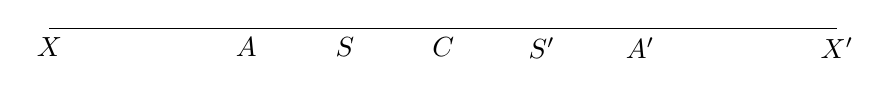
\begin{tikzpicture}[scale=1.25]

\coordinate (X) at (0,0);
\node[below] at (X) {$X$};
\vertexsm{X};
\coordinate (A) at (2,0);
\node[below] at (A) {$A$};
\vertexsm{A};
\coordinate (S) at (3,0);
\node[below] at (S) {$S$};
\vertexsm{S};
\coordinate (C) at (4,0);
\node[below] at (C) {$C$};
\vertexsm{C};
\coordinate (SP) at (5,0);
\node[below] at (SP) {$S'$};
\vertexsm{SP};
\coordinate (AP) at (6,0);
\node[below] at (AP) {$A'$};
\vertexsm{AP};
\coordinate (XP) at (8,0);
\node[below] at (XP) {$X'$};
\vertexsm{XP};

\draw (X) -- (XP);

\end{tikzpicture}
\end{center}

%%%%%%%%%%%%%%%%%%%%%%%%%%%%%%%%%%%%%%%%%%%%%%%%%%%%%%%%%%%%%

\begin{theorem}
\begin{equation}
\frac{SA}{AX}=\frac{AA'}{XX'}\,.\label{eqn.cacx}
\end{equation}
\end{theorem}

\begin{proof}
From the diagram we have
\begin{eqn}
\frac{AA'}{SA}-1&=&\frac{AA'}{SA}-\frac{SA}{SA}=
\frac{AA'-SA}{SA}=\frac{SA'}{SA}\\[8pt]
\frac{XX'}{AX}-1&=&\frac{XX'}{AX}-\frac{AX}{AX}=
\frac{XX'-AX}{AX}=\frac{AX'}{AX}\,.
\end{eqn}
But $A,A'$ are both points on the ellipse so
\begin{eqn}
\frac{SA'}{AX'}&=&\frac{SA}{AX}\\[4pt]
\frac{SA'}{SA}&=&\frac{AX'}{AX}\\[4pt]
\frac{AA'}{SA}&=&\frac{XX'}{AX}\,.\fqed
\end{eqn}
\end{proof}

%%%%%%%%%%%%%%%%%%%%%%%%%%%%%%%%%%%%%%%%%%%%%%%%%%%%%%%%%%%%%

\begin{theorem}
$SP+S'P = AA'$.
\end{theorem}

%%%%%%%%%%%%%%%%%%%%%%%%%%%%%%%%%%%%%%%%%%%%%%%%%%%%%%%%%%%%%

\begin{figure}[b]
\begin{center}
\begin{tikzpicture}
\clip (-4.6,-2.2) rectangle +(9.2,4.6);
% Ellipse
\def\a{3}
\def\b{2}
\pic{ellipse={{\a}/{\b}}};

% Label nodes
\node[below right] at (Right) {$A'$};
\node[below left] at (Left) {$A$};
\node[below] at (F1) {$S$};
\node[below] at (F2) {$S'$};
\node[below left,xshift=3pt,yshift=-2pt] at (O) {$O$};

\coordinate (X) at (-4,0);
\node[below left] at (X) {$X$};
\draw (Left) -- (X) -- +(0,{\b});
\draw (X) -- +(0,{-\b});
\coordinate (XP) at (4,0);
\node[below right] at (XP) {$X'$};
\draw (Right) -- (XP) -- +(0,{\b});
\draw (XP) -- +(0,{-\b});

% Indicates distances along the major axis
\draw[<->] ($(O)+(0,-20pt)$) -- node[fill=white] {$a$} ($(Right)+(0,-20pt)$);
\draw[<->] ($(O)+(0,-20pt)$) -- node[fill=white] {$a$} ($(Left)+(0,-20pt)$);

\def\angle{110}
\coordinate (P) at ({\angle}:{\a} and {\b});
\path[name path global=fromF1p] (P) -- (F1);
\path[name path=ph] (P) -- (F2);
\path[name path global=pc] (P) -- (O);
\node[above left] at (P) {$P$};
\draw[thick,red] (F1) -- (P) -- (F2);
\coordinate (N) at (P|-O);
\draw[thick,blue] (P) -- (N) node[below,black] {$N$};
\draw[blue,thick] (N) rectangle +(7pt,7pt);

\draw[thick,dashed] (P-|X) node[left] {$K$} -- (P-|XP) node[right] {$K'$};

\end{tikzpicture}
\caption{$SP+SP'=AA'$}
\label{f.AAP}
\end{center}
\end{figure}

%%%%%%%%%%%%%%%%%%%%%%%%%%%%%%%%%%%%%%%%%%%%%%%%%%%%%%%%%%%%%

\begin{proof}
Let $N$ be the perpendicular from $P$ to the major axis (Figure~\ref{f.AAP}). $P$ is on the ellipse if $SP/PK=e$ or $SP'/PK'=e$, but since $PK=NX$ and $PK'=NX'$, $P$ is on the ellipse if $SP/NX=e$ or $SP'/NX'=e$.
\begin{eqn}
\frac{SP}{NX}&=&\frac{SP'}{NX'}\\[4pt]
\frac{SP'}{SP}&=&\frac{NX'}{NX}\\[4pt]
\frac{SP'+SP}{SP}&=&\frac{NX'+NX}{NX}\\[4pt]
\frac{SP'+SP}{SP}&=&\frac{XX'}{NX}\,.
\end{eqn}
Again since $P$ is on the ellipse and by Equation~\ref{eqn.cacx},
\begin{eqn}
\frac{SP'+SP}{XX'}&=&\frac{SP}{NX}=\frac{SA}{AX}=\frac{AA'}{XX'}\\[4pt]
SP'+SP&=&AA'\,.\fqed
\end{eqn}
\end{proof}

